\documentclass[a4paper]{article}

\usepackage{hyperref}
\usepackage{amsmath}
\usepackage[noend]{algpseudocode}
\usepackage{xcolor}
\usepackage{graphicx}
\usepackage[font={small}]{caption}
\usepackage[toc,page]{appendix}

% Times font
\usepackage{mathptmx}

\renewcommand{\figurename}{\bf Figure}

\bibliographystyle{ieeetr}

\title{An Adaptive Just Intonation Algorithm for Barbershop Music}
\author{{\bf Teun Buwalda}\\t.c.buwalda@students.uu.nl\\6787886, Utrecht University\\Bachelor's thesis}

\begin{document}
\maketitle

% Thanks:
% Jeroen en Peter
% Jos en Tijs
% Marc en Than
% Jasper en Jay

% TODO: Abstract
\begin{abstract}
	{\color{red}Hier komt dus waarschijnlijk nog een abstract.}
\end{abstract}

\section{Introduction}
The piano is out of tune. Most modern music is tuned to \textit{equal temperament}, in which every musical interval (i.e. distance between two tones) is slightly too small or too big in the standard tuning of the piano. \cite{van_de_craats_fis_1989} Music groups that have the possibility to, can attempt to alter their intonation according to \textit{just intonation} instead, approximating simple mathematical frequency ratios. \cite{fonville_ben_1991} Barbershop quartets, for instance, explicitly try to achieve just intonation on every chord. \cite{barbershop_harmony_society_contest_2022, averill_bell_1999}

However, when a singer holds a note across multiple chords, there is no unbiased answer as to how exactly each note should be tuned. Holding the note at exactly the same pitch can either require a deviation from just intonation or an overall pitch drifting effect over time. \textit{Adaptive tuning systems} are algorithms that tune each playing note such that they approximate just intonation. The choices that these systems have to deal with, are explored further in paragraph \ref{intro_adaptive_ji}.

This thesis project will answer two separate questions. Question A concerns the solution to barbershop quartets' problem: {\it what adaptive tuning algorithm would a mathematically ideal barbershop quartet follow, given a score?} In this first part of the thesis, an adaptive tuning system for barbershop music will be proposed. It will optimise four criteria (outlined in Section \ref{methodoloy}) which are important to the genre. In order to validate the algorithm, the Results section will show how the algorithm accounts for these four criteria and where concessions need to be made in order to minimise conflicts between them.

Research question B is: {\it can we implement the tuning system from question A so that it models the ideal barbershop quartet?} This second part of the project should result in a C$\sharp$ program that, given a sequence of chords, can play them back justly tuned and following the genre's limitations, possibly serving as a suggestion for performers and allowing for high-level analysis of the algorithm's performance in Section \ref{results}.

Despite the extensive research into adaptive tuning systems, an algorithm that takes the limitations of barbershop quartets into account, such as the roles of the four different voices, is not known to have been made to the author. Adaptive tunings generally do not model human choirs, as their main purpose is to provide a way in which all music can be played back in tune. Most previous work in adaptive just intonation therefore takes a general approach, maximising dynamicity in trying to work for every performer, but they are not quite applicable to barbershop. Therefore, this thesis project adds a new dimension to the field of adaptive just intonation. At the same time, methods from Hermode Tuning \cite{mohrlok_hermode_2003} and Pivotuner \cite{volkov_pivotuner_2022} are important inspirations for the solution to research question A.

To provide the necessary context to answer both of these questions, the following section will expand upon the subjects of just intonation, adaptive just intonation algorithms and barbershop music. The following section will describe the exact methodology and further describe the algorithm's constraints. Sections \ref{algorithm} and \ref{implementation} will answer research questions A and B, respectively. Section \ref{results} will attempt to evaluate the algorithm by analysing results such as global pitch drift and particularly hard-to-tune passages. Section \ref{discussion} will then place this research in the context of other literature about choirs, tuning and philosophy.

\section{Theoretical Framework}
\subsection{Just Intonation}
\label{intro_ji}

\begin{figure}
	\centering
	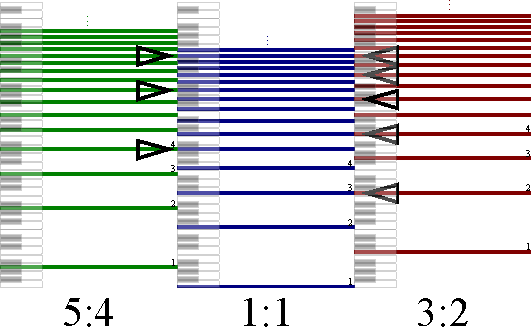
\includegraphics{Figures/overtones.pdf}
	\caption{The relationship between just intonation and the overtone series, which is the cause of the "lock and ring" effect as pursued by barbershop musicians. The figure shows three tones with their respective overtones, the harmonic frequencies that create the sound's timbre. A piano keyboard was overlaid for pitch reference. The A (left, green) is tuned a just major third above the F (middle, blue), which makes the A's 4th, 8th and 12th overtone share the exact frequency of the F's 5th, 10th and 15th. The C (right, red) is tuned to a just fifth above the F, which means every one of its overtones which is a multiple of 2 shares its frequency with one of the F's overtones which is a multiple of 3. Because of these shared overtones, the chord has a stable sound, minimising interference by close-but-not-quite-the-same frequencies.}
	\label{fig:overtones}
\end{figure}

In many musical contexts, {\it just intonation} is seen as the ideal method for tuning. \cite{boyden_prelleur_1951} Rather than predefining each tone's pitch, like necessary when tuning an instrument such as the piano, just intonation defines specific frequency ratios for each musical interval. The most common intervals are the octave (defined as $2:1$), the fifth ($3:2$) and the major third ($5:4$). For example, if an A is tuned at $220$ Hz, then an E a fifth above this A will be tuned at $220 \cdot \frac32 = 330$ Hz. The minor seventh, which is also prevalent in barbershop music \cite{barbershop_harmony_society_contest_2022}, is defined as $7:4$. \cite{van_de_craats_fis_1989} These ratios are different from the tuning system used by most modern pianos.

The ratios are drawn from the smallest intervals of the \textit{harmonic series}, which refers to the set of overtones that can be heard above nearly every sung, played or synthesised tone. When musical intervals follow these simple ratios, the overtones of different tones "lock together" and create a specific auditory experience that many musicians strive for. This sound is caused by the fact that tones that share a simple ratio will also share many overtones (Figure \ref{fig:overtones}). Because of these shared overtones, the different tones barely interfere with each other, creating a more stable sound.

Sadly, it is mathematically impossible to devise fixed pitches for a set of twelve tones such that each pair of tones always exactly follows one of the simple ratios from just intonation. A consequence of this fact is that it is also impossible to provide a "perfect" tuning for the piano. This impossibility is demonstrated with the example in Figure \ref{fig:thirdsproof}, which shows two different ways to walk from a low C to a high C. Suppose we want the major third to be equal to 4 semitones, as is the case in western music theory \cite{forte_tonal_1979}, then a major third should sound between C and E, between E and G$\sharp$ and between G$\sharp$ and a high C. The major third has a ratio of $5:4$. Then the ratio between a low C and E on the piano should be $5:4$, as should the ratio between E and G$\sharp$ and the ratio between G$\sharp$ and a high C. Therefore, the ratio between the low C and G$\sharp$ should be $\frac54 \cdot \frac54 = \frac{25}{16}$ and the ratio between the low C and the high C should be $\frac{25}{16} \cdot \frac54 = \frac{125}{64}$. However, the two Cs are also one octave apart and should therefore have a ratio of $\frac21$. These two ratios are not the same, which shows that it is impossible to devise a tuning system such that both major thirds and octaves are always in tune according to just intonation.

\begin{figure}
	\centering
	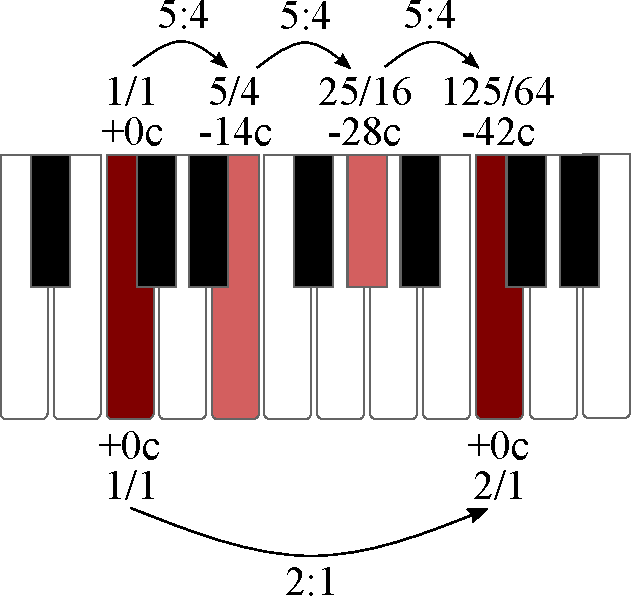
\includegraphics[width=0.6\linewidth]{Figures/ThirdsProof.pdf}
	\caption{12 fixed tones are not compatible with just intonation. For each coloured tone, its frequency ratio with the low C is written. The difference with equal temperament in cents is also written. The bottom path shows that a high C should be tuned at exactly twice the frequency of the low C when tuning the octave justly. The top path instead uses justly tuned major thirds with the standard $5:4$ ratio. The two paths come out at a different tuning for the high C, proving that major thirds and octaves are incompatible.}
	\label{fig:thirdsproof}
\end{figure}

Most modern music accepts the fact that just intonation cannot be achieved, using equal temperament as a substitute. In twelve-tone equal temperament, the octave is divided into twelve logarithmically equal divisions. Since the octave is defined by the frequency ratio $2:1$, this custom puts the smallest interval (the semitone) at exactly $\sqrt[12]{2}:1$. \cite{van_de_craats_fis_1989} For example, if an A is tuned at $220$ Hz, then the lowest tone above this A, a B$\flat$, will be tuned at $220\cdot \frac{\sqrt[12]{2}}{1} \approx 233.08$ Hz. Figure \ref{fig:12TET} shows the standard tuning in equal temperament for a part of the piano keyboard. Twelve-tone equal temperament works relatively well for some intervals, such as the fifth, which is only slightly too small compared to just intonation. On the contrary, intervals like the major third and the minor seventh are significantly smaller in just intonation than in equal temperament.

\begin{figure}
	\centering
	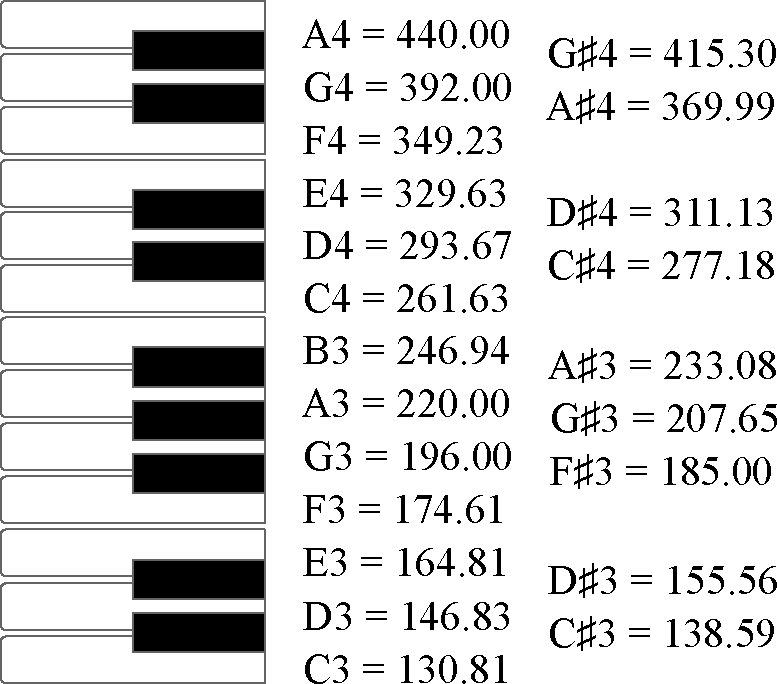
\includegraphics[width=0.65\linewidth]{Figures/12TET.pdf}
	\caption{A selection of standard frequency values for piano in equal temperament, shown in Hertz. Equal temperament is the most common tuning method and ensures that each semitone is always the same relative size, namely $\sqrt[12]{2}:1$. However, just intonation is not compatible with equal temperament; for example, if this E4 were tuned to a perfect fifth ($3:2$) with the A3 according to just intonation, it should be $330.00$ Hz, which is slightly higher than it is in equal temperament.}
	\label{fig:12TET}
\end{figure}

When talking about the difference between just intonation and 12-tone equal temperament, the \textit{cent} interval is often used as a unit. 1 cent is defined as $\frac{1}{100}$ of a semitone in equal temperament, meaning it has a frequency ratio of $\sqrt[1200]{2}:1$. A justly tuned major third, for example, is 14 cents lower than a major third in equal temperament (Figure \ref{fig:thirdsproof}).

\textit{Note about terminology.} The addition of the cent interval leaves us with three different ways to describe a tone's exact tuning: in Hertz, with a fraction or in cents. Hertz makes the most sense in physics: an A3 can be tuned at 220 Hz, whereas an E4 would be tuned at 329.63 Hz on the piano. In just intonation, we often use fractions: when tuning an E4 to be a perfect fifth above this A3, the E4's tuning would need to be $\frac32$ times the frequency of the A3 (equivalently, 330.00 Hz). The cent interval puts this abstract difference in perspective: 330.00 Hz is 2 cents higher than 329.63 Hz, meaning $\frac{2}{100}$ of a semitone.

\subsection{Adaptive Just Intonation Systems}
\label{intro_adaptive_ji}
Although just intonation is impossible to achieve when all twelve tones have a fixed tuning, such as on an acoustic piano, it can be achieved when using instruments that can \textit{adaptively} tune specific notes. In other words, if a note can be tuned differently based on which other notes are playing, the strict mathematical ratios of just intonation can be followed. This idea is, for example, applied to ensembles with human voices, string instruments such as the violin, or trombones, since all of those instruments can continuously change their pitch by ear. \cite{van_de_craats_fis_1989}

Modern computational techniques also allow digital instruments to be tuned adaptively. Much research has been done into automatic \textit{adaptive tuning systems}: programs that take sets of musical notes as input, and return their respective tunings according to just intonation as output. Sethares \cite{sethares_adaptive_1994} approached the problem very generally by minimising a loss function based on a sound's dissonance curve. Løberg (2002) implemented a dynamic tuning system by the Norwegian composer Eivind Groven that dynamically chooses between 36 available tones to get just intervals. \cite{code_grovenmax_2002} Commercial software such as Hermode Tuning \cite{mohrlok_hermode_2003} and Pivotuner \cite{volkov_pivotuner_2022} can be integrated into music software to retune all played notes based on the sounding chord. Hermode sums the deviations in cents from equal temperament of all sounding notes and ensures that the result is mostly equal to 0. Conversely, Pivotuner picks a single note in each chord that should remain at the same pitch, enabling an artistic use of the resulting tonal centre drift.

However, adaptive just intonation does not have a single algorithm that completely solves the mathematical problem of tuning. Choices need to be made with regards to optimisation of melodic intervals, held notes and tonal centre drift. Optimisation of melodic intervals means that the intervals within the melody follow equal temperament as much as possible. Optimisation of held notes means notes that keep sounding in different chords do not need to be dramatically retuned for each new chord. Tonal centre drift is a gradual lowering or heightening of the average tuning of notes, which is generally seen as undesirable. \cite{dougherty_choral_2004, barbershop_harmony_society_contest_2022} If held notes are allowed to retune freely, just intonation without pitch drift is possible. To achieve this goal, the performance can make sure the melody always follows equal temperament intervals and the other voices change their pitches to tune justly with the melody. \cite{dougherty_choral_2004} In contrast, the constraint of held notes staying at the same pitch between different chords causes problems.

To illustrate this incompatibility of the held notes constraint with the other constraints, consider a C major triad (C-E-G) moving to an E major triad (E-G$\sharp$-B), with the E being held between the two chords. If the C is tuned according to equal temperament (i.e. $261.6$ Hz), then the E will have to be 2.6 Hz lower than equal temperament in order to create the standard $5:4$ ratio of the major third (as $261.6 \cdot \frac54 = 327.0$ Hz, rather than $329.6$ Hz). If this lower E is held into the next chord, then the G$\sharp$ and B will also be tuned lower to tune justly with the E. Therefore, the overall tonal centre has moved 2.6 Hz downwards ("flat"). This downward shift shows that held notes and tonal centre drift cannot both be optimised at the same time.

\subsection{Barbershop Music}
\label{intro_bs}
% barbershop in 1 alinea
% barbershop en just intonation
% de barbershopregels die just intonation moeilijker maken
Barbershop is a distinct genre of four-part singing that is most prevalent in North America. The music is primarily sung in quartets, though larger choirs are also often formed, of which quartets form smaller subsets. \cite{garnett_ethics_1999} The Barbershop style is very specifically defined and has an active community that aims to preserve the genre according to its general definition. Some of the largest central events where Barbershop enthusiasts gather are competitions, where quartets are judged according to this specific definition. In this paper, the Barbershop Harmony Society's definition of barbershop music and its Contest and Judging Handbook \cite{barbershop_harmony_society_contest_2022} will often be cited as the main source of information about priorities within the genre.

In this official definition, barbershop music is described as having four voices: tenor, lead, baritone and bass. The lead generally sings the melody, but exceptions can occur within a song. The melody is accompanied by mostly homorhythmic (i.e. in the same rhythm as the lead) harmonies in the other three voices. Chords generally do not get too complicated: most songs revolve around major and minor chords without many harmonic extensions. \cite{barbershop_harmony_society_contest_2022} Additionally, the dominant seventh chord is often described as the most important chord in barbershop music. \cite{averill_bell_1999}

The Contest and Judging Handbook (page 7-2, paragraph II.A.) describes just intonation as one of the key elements of barbershop music. It prescribes tuning in barbershop music as follows:
\begin{quote}
	Barbershop singers adjust pitches to achieve perfectly tuned chords, and yet sing a melodic line that remains true to the tonal center. Barbershop singers strive for more precise tuning than is possible with the fixed 12-tones- per-octave of the equally tempered scale of fixed-pitched instruments, such as the piano. Essentially, we use just intonation for harmonic tuning while remaining true to the established tonal center. \cite{barbershop_harmony_society_contest_2022}
\end{quote}
Barbershop singers try to minimise "beats" in the sound of their harmonies, the auditory artefacts that appear when chords are not tuned justly. When quartets follow interval ratios as described in \ref{intro_ji}, the overtones of the different parts match and create a buzzing, unchanging auditory experience that is described as "lock and ring".

However, very few barbershop quartets consistently achieve the high standard of just intonation. \cite{garnett_ethics_1999} The above quote immediately describes one of the major dilemmas that singers face when attempting to follow just intonation: tonal centre drift (see \ref{intro_adaptive_ji}). Besides attempting to maintain a constant tonal centre, quartets may also try to have the lead follow consistent melodic intervals similar to those on the piano, and refrain from moving held notes around too much.

\subsection{Relevance to KI}
This thesis project is part of the bachelor Kunstmatige Intelligentie at Utrecht University. The Utrecht University AI programmes focus on Human-Centered Artificial Intelligence (HCAI), rather than trying to keep up with the latest innovations in machine learning algorithms. HCAI targets to understand, reproduce and if possible enhance human intelligence. \cite{utrecht_university_human-centered_2023} Modelling something specifically human such as music is inherently AI research, especially when trying to build an algorithm that is inspired by human performance, but performs better. Therefore, finding a tuning algorithm for barbershop music fits right into the HCAI focus area.

\section{Methodology}
\label{methodoloy}
% Nog eens een algemene omschrijving van wat het algoritme moet doen
% input (language, including chords)
  % fractions input
% output: MIDI, but also analysis
This paper will propose an algorithm that adaptively tunes barbershop scores to just intonation. Figure \ref{fig:pipeline} shows the pipeline that the algorithm should follow. The tuning system will optimise the following criteria:
\begin{enumerate}
	\item maintain just intonation on every chord [\textit{just intonation constraint}]
	\item account for the different roles of the four parts: specifically, the lead's intervals should mostly stick to 12-tone equal temperament [\textit{lead constraint}]
	\item minimise (but not necessarily eliminate) retuning of held notes [\textit{tie constraint}]
	\item minimise (but not necessarily eliminate) tonal centre drift [\textit{drift constraint}]
\end{enumerate}

\begin{figure}
	\centering
	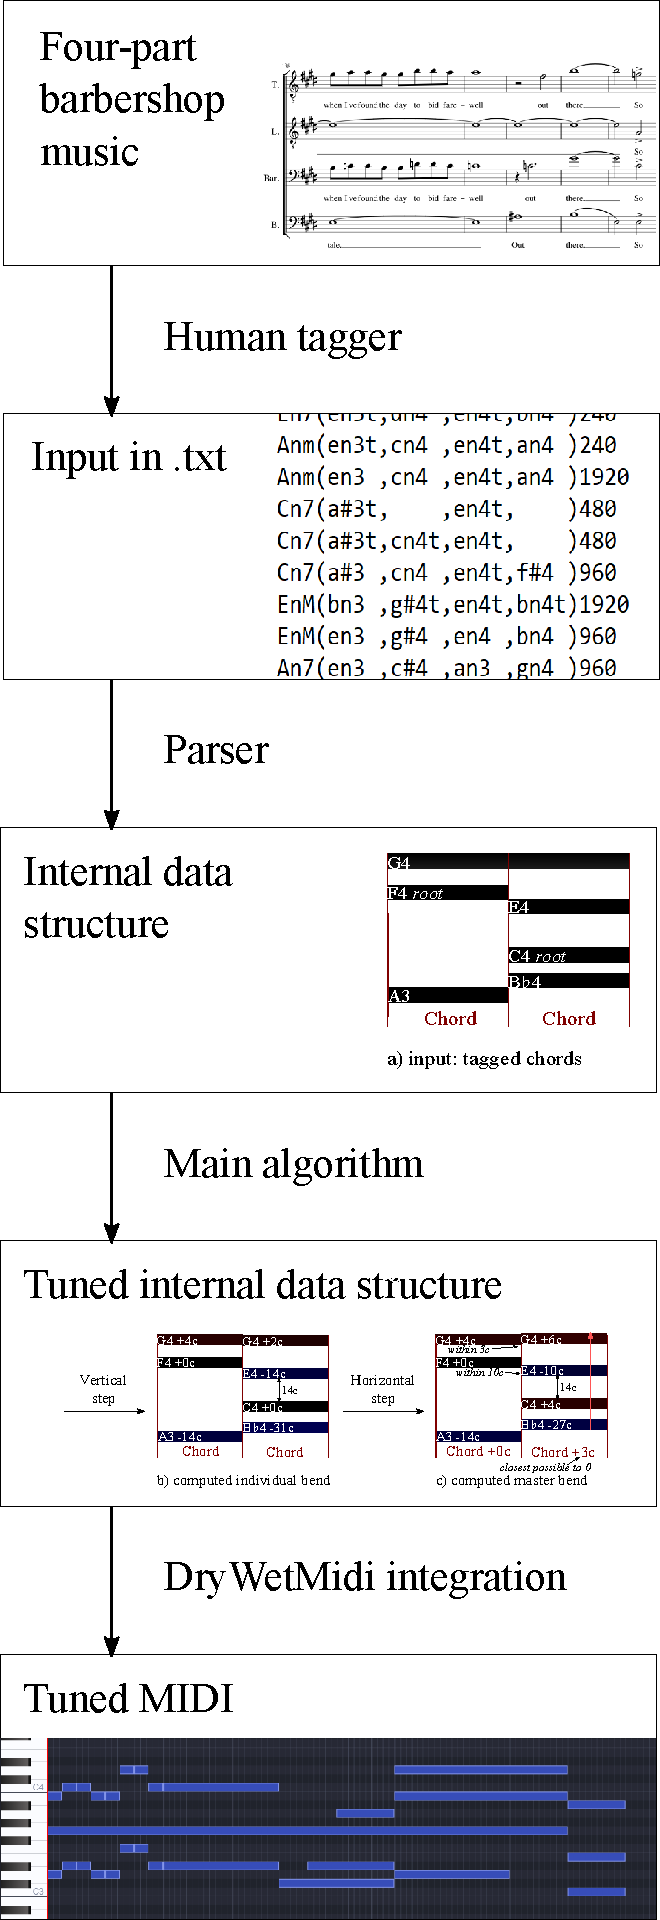
\includegraphics[width=0.5\linewidth]{Figures/pipeline.pdf}
	\caption{Pipeline for an adaptive just intonation algorithm for barbershop music. The program works on any four-part score, but requires a human tagger to translate it into a language that is specific to this algorithm. A parser can then interpret this language and build the internal data structure that the main algorithm uses to determine how each note should be tuned. At last, the library DryWetMidi is used to convert the tuned internal data structure to a MIDI file with pitch bend messages.}
	\label{fig:pipeline}
\end{figure}

The input of the algorithm consists of \verb+.txt+ files that describe a barbershop score. The \verb+.txt+ files should be written using a newly-defined language specific to this project that contains information about note pitches, harmonies, tied notes and durations. This language is described in Appendix \ref{input}. Importantly, the input splits the score into \textit{Chords}, which in this case are periods of time where none of the notes change. A new Chord begins any time one of the four voices stops singing, starts singing or moves to a different pitch. Figure \ref{fig:algo_outline} visualises such a split score.
% TODO betere figuur hier

Because of this newly-defined language, a parser must be programmed to convert the input \verb+.txt+ files into the program's internal data structure. Conversion from the original sheet music to the input language is, for now, a human job.

The output of the algorithm consists of a MIDI file \cite{midi_manufacturers_association_complete_2014} and some general statistics such as how much the song had to drift in general and which chords caused the most dramatic retunings. The MIDI files mostly contain the original notes from the score, now with extra pitch bend messages. Section \ref{implementation} will describe the MIDI conversion in further detail.


\section{Algorithm}
\label{algorithm}
% indivBend vs masterBend
% describe vertical step
% describe horizontal step
% parameters
This section will describe the tuning algorithm proposed by this paper, thereby answering research question A: {\it what adaptive tuning algorithm would a mathematically ideal barbershop quartet follow, given a score?} The algorithm returns a set of bend values that prescribe how much each note in the song should deviate from 12-tone equal temperament. The algorithm consists of a vertical step and a horizontal step. The vertical step satisfies the just intonation constraint from Section \ref{methodoloy}, whereas the horizontal step satisfies the other three constraints. The vertical step is a relatively standard procedure for just intonation, whereas the horizontal step is a completely new proposal. Figure \ref{fig:algo_outline} shows an outline of the full algorithm.

\begin{figure}
	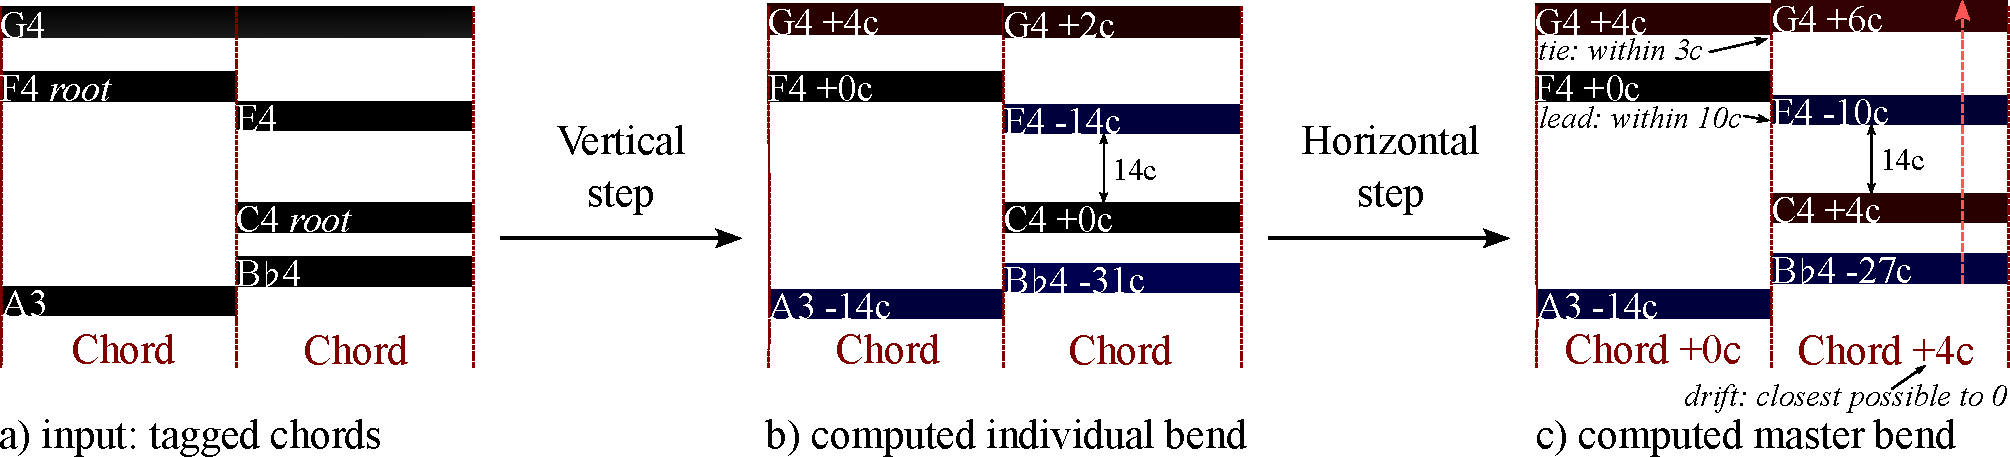
\includegraphics[width=\linewidth]{Figures/algo_outline.pdf}
	\caption{A basic view of the algorithm. tieRange = 3c, leadRange = 10c. The vertical step tunes each note separately, relatively to each other (\textit{individual bend}), satisfying the just intonation constraint. The horizontal step then attempts to satisfy the tie, lead and drift constraints by moving all notes in the chord at the same time (\textit{master bend}).}
	\label{fig:algo_outline}
\end{figure}

The algorithm distinguishes between two levels of tuning: \textit{individual bend} and \textit{master bend}. The individual bend describes how much the notes within a chord differ from each other and is determined in the vertical step of the algorithm. A note's individual bend is only relative to the tuning of the other three notes in the chord, where a chord only spans a period of time where not a single note changes. The master bend, on the other hand, is used to move an entire chord's tuning up or down and is determined in the horizontal step. A note's pitch is ultimately calculated by adding its individual bend to the chord's master bend (\textit{posterior bend}) and using the result as a degree of deviation from just intonation. Importantly, a note's individual bend never changes after the vertical step of the algorithm is done, making sure the notes of one chord always stay justly tuned with one another. Therefore, constraint 1 is always satisfied.

The vertical step (Figure \ref{fig:algo_outline}b) determines each note's individual bend using just intonation intervals. The bend value for the chord root is always set to 0 (again, since these are relative values, that does not actually mean the root will be tuned to the regular 12-tone equal temperament value). The bend values for the other playing notes are decided using a set of interval values based on fractions relative to the chord root. This set of fractions can be given by the user, but a standard set is provided. The fractions are taken from simple ratios in the harmonic series. For example, the dominant seventh chord is usually described with a $4:5:6:7$ ratio between its chord tones. Therefore, in an A dominant seventh chord (A-C$\sharp$-E-G), the G's frequency will be tuned to be $\frac74$ times the A's frequency. On the other hand, a half-diminished chord is usually described with a $5:6:7:9$ ratio, so in an A half-diminished chord (A-C-E$\flat$-G), the G will be equal to $\frac95$ times the A.

The horizontal step (Figure \ref{fig:algo_outline}c) moves all chord notes around evenly to satisfy constraints 2-4 (lead, tie and drift; see Section \ref{methodoloy}). Specifically, it outputs a master bend value for the current chord by comparing it to the previous chord. For the lead and tie constraints, a collection of lead notes and tied notes from the previous chord is made in order to calculate how much the current master bend can move around while satisfying those constraints. Each of those notes has a desired space that the new note should move into. To illustrate: in the example, $\mathit{tieRange}$ is set to 3 and the previous G4 is tied over, so the current G4 should be within 3 cents of the old G4. Meanwhile, $\mathit{leadRange}$ is set to 10 and the previous F4 has a posterior bend of 0 cents, so the current E4 should deviate less than 10 cents from equal temperament. After the collection of lead and tied notes has been completely run through, the algorithm chooses a value for the master bend that is as close to 0 as possible. This last step helps the drift constraint, because a master bend value of 0 means that there is no tonal centre drift.

Ultimately, the algorithm's results depend on a set of parameters given by the user. The first parameter is a set of lists of fractions that should be used for the vertical step. This first parameter is important to note, because opinions vary as to which exact tunings are the best for each interval. The other three parameters are referred to as $\mathit{priority}$, $\mathit{tieRange}$ and $\mathit{leadRange}$. $\mathit{priority}$ is either "lead" or "tie" and determines whether the lead or tie constraint should be satisfied first. $\mathit{tieRange}$, given in a unit similar to cents, determines how much a tied note is allowed to be retuned compared to its predecessor. $\mathit{leadRange}$ is similar: it determines by how many cents an interval in the lead voice is allowed to deviate from an interval in equal temperament, relatively. For instance, if $\mathit{tieRange}$ is set to 3 and $\mathit{priority}$ is set to "tie", the horizontal step of the algorithm will prioritise moving the most important tied note less than 3 cents up or down over the other tied notes, the lead constraint and the drift constraint.

\section{C$\sharp$ Implementation}
\label{implementation}
Now that Section \ref{algorithm} has described the just intonation algorithm for barbershop music, we can look at how the algorithm was implemented into the programming language C$\sharp$. This section therefore answers research question B: {\it can we implement the tuning system from question A so that it models the ideal barbershop quartet?}

\textit{\color{red}Dit moet ik nog schrijven. Als jullie deze week al vragen hebben over de implementatie hoor ik het graag!}

% Classes: Notes with indivBend, Chords with masterBend, Song and BSTuner to tie it all together
% Vertical step implementation, \ref{input_fractions}
% Horizontal step implementation w/ pseudocode
% MIDI (and analysis) output, with library DryWetMidi: 4 bend messages on each Chord

\begin{figure}
	\begin{algorithmic}[1]
		\Procedure{SetMasterBend}{$\mathit{MB}_{i-1}, \mathit{Notes}_{i-1}, \mathit{Notes}_i, \mathit{tieRange}, \mathit{leadRange}$}
		\State $\mathit{ties} \gets [$all notes in $\mathit{Notes}_{i-1}$ that have the tie property, ordered lead-bass-tenor-baritone$]$
		
		\State $\mathit{ranges} \gets [$for all tied notes, the range $\mathit{MB}_i$ could move into in order to satisfy its parameter$]$
		\State $\mathit{ranges.Add}($the range in which $\mathit{MB}_i$ could move according to $\mathit{leadDiff})$
		
		\If{0 is within $\bigcap \mathit{ranges}$}
		\State\Return{$\mathit{MB}_i \gets 0$}
		\Else
		\State $\mathit{currRange} \gets \mathit{ranges}[0]$
		\ForAll{$\mathit{range} \; r \; in \;  \mathit{ranges}[1:]$}
		\State $\mathit{currRange} \gets r \cap \mathit{currRange}$
		\If{no intersection}
		\State \Return{$\mathit{MB}_i \gets$ the closest number to $r$ within $\mathit{currRange}$}
		\EndIf
		\EndFor
		
		\State\Return{$\mathit{MB}_i \gets$ the closest number to 0 within $\mathit{currRange}$}
		\EndIf
		\EndProcedure
	\end{algorithmic}
	\caption{Pseudocode for the horizontal step. The input is two Chords, both of which contain four notes. The output is a master bend value for the current chord which takes the tie, lead and drift constraints into account. The just intonation constraint has already been completely satisfied by the vertical step. \textit{\color{red}Hier komt nog meer uitleg, hoort bij het implementatie-hoofdstuk}}
	\label{fig:pseudocodeH}
\end{figure}

\section{Results}
\label{results}
% algemeen: laat zien hoe het algoritme reageert op een stukje voorbeeldmuziek. Daarbij is dus bladmuziek nodig met annotaties (MScore naar PDF exporteren, dan in Inkscape erbij tekenen). Liefst een stukje waar het dan ook echt bij moet driften voor bepaalde parameters (probeer er een paar uit en laat alles zien).
% Ik ga hier de tag van Ring-A Ding Ding voor gebruiken
% Grafieken vanuit R met effecten op parameters

% Om te zien hoe dit algoritme het doet: stukje voorbeeldmuziek met verschillende parameters
% We gebruiken dit nummer, is interessant voor deze redenen (bv. 2 lange tied noten, zoals vaak in tags)
This section will show the proposed algorithm's effect on an example score, namely the tag of \textit{Ring-a-Ding-Ding}, arranged by Anthony Bartholomew. Several good recordings of this song can be found on \href{https://www.youtube.com/watch?v=G40I5JDtfjI&t=147s}{YouTube}. Figure \ref{fig:ding_sheets} shows the sheet music for this tag. Since both the bass and tenor voices hold notes for a long time while the lead and baritone sing phrases in-between, \textit{Ring-a-Ding-Ding} is a good example to show how the proposed algorithm makes choices in ambiguous scenarios. This paper's \href{https://github.com/teuncb/adaptivebarbershop}{GitHub page} also contains the algorithm's output MIDI files for \textit{Ring-a-Ding Ding}, as well as the results from other barbershop snippets, so it is possible to listen and compare.

Figure \ref{fig:results} shows the effects that the three parameters (tieRange, leadRange and priority, see \ref{algorithm}) have on the lead, tie and drift constraints in \textit{Ring-a-Ding-Ding}. Note that the just intonation constraint is, because of the permanent nature of the vertical step, always satisfied. The lead constraint is quantified as the number of lead intervals that had to deviate more than 10 cents from equal temperament intervals. The tie constraint is quantified as the number of pairs of held notes where the second note was more than 3 cents higher or lower than the first. The overall tonal centre drift with these parameters has also been plotted.

% ranges ~ drift, flinke sprong nadat range de bar overschrijdt, prio niet zoveel effect (ws soms 1 noot), 
The plots show that tonal centre drift is negatively correlated with both $\mathit{Range}$ parameters: if notes and intervals are allowed to differ more from the ideal changes, then the song will drift less. Specifically, a stricter $\mathit{tieRange}$ causes less pitch drift earlier than a stricter $\mathit{leadRange}$ for this song. Since an "audible retuning" is set to be at least 3 cents, the number of audible retunings leaps after the $\mathit{tieRange}$ passes 3 cents. The song only needs to deviate from equal temperament in lead intervals a couple of times, which is why this leap is invisible in the red line. When the $\mathit{priority}$ is set to "lead", not a single deviation from equal temperament is necessary and the number of tied note retunings is relatively low in general.

\begin{figure}
	\centering
	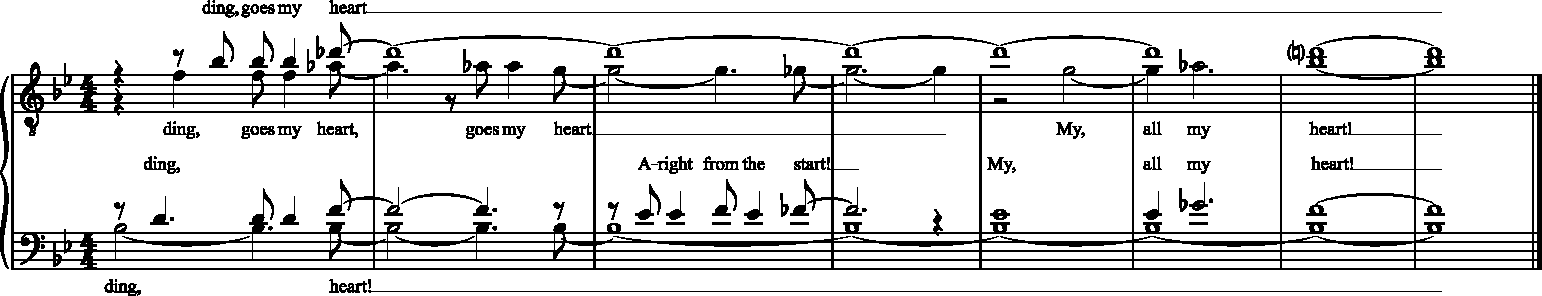
\includegraphics[width=\linewidth]{Figures/Ding_MuseScore.pdf}
	\caption{Sheet music for the tag of Ring-a-Ding-Ding, a barbershop arrangement by Anthony Bartholomew.}
	\label{fig:ding_sheets}
\end{figure}

\begin{figure}
	\centering
	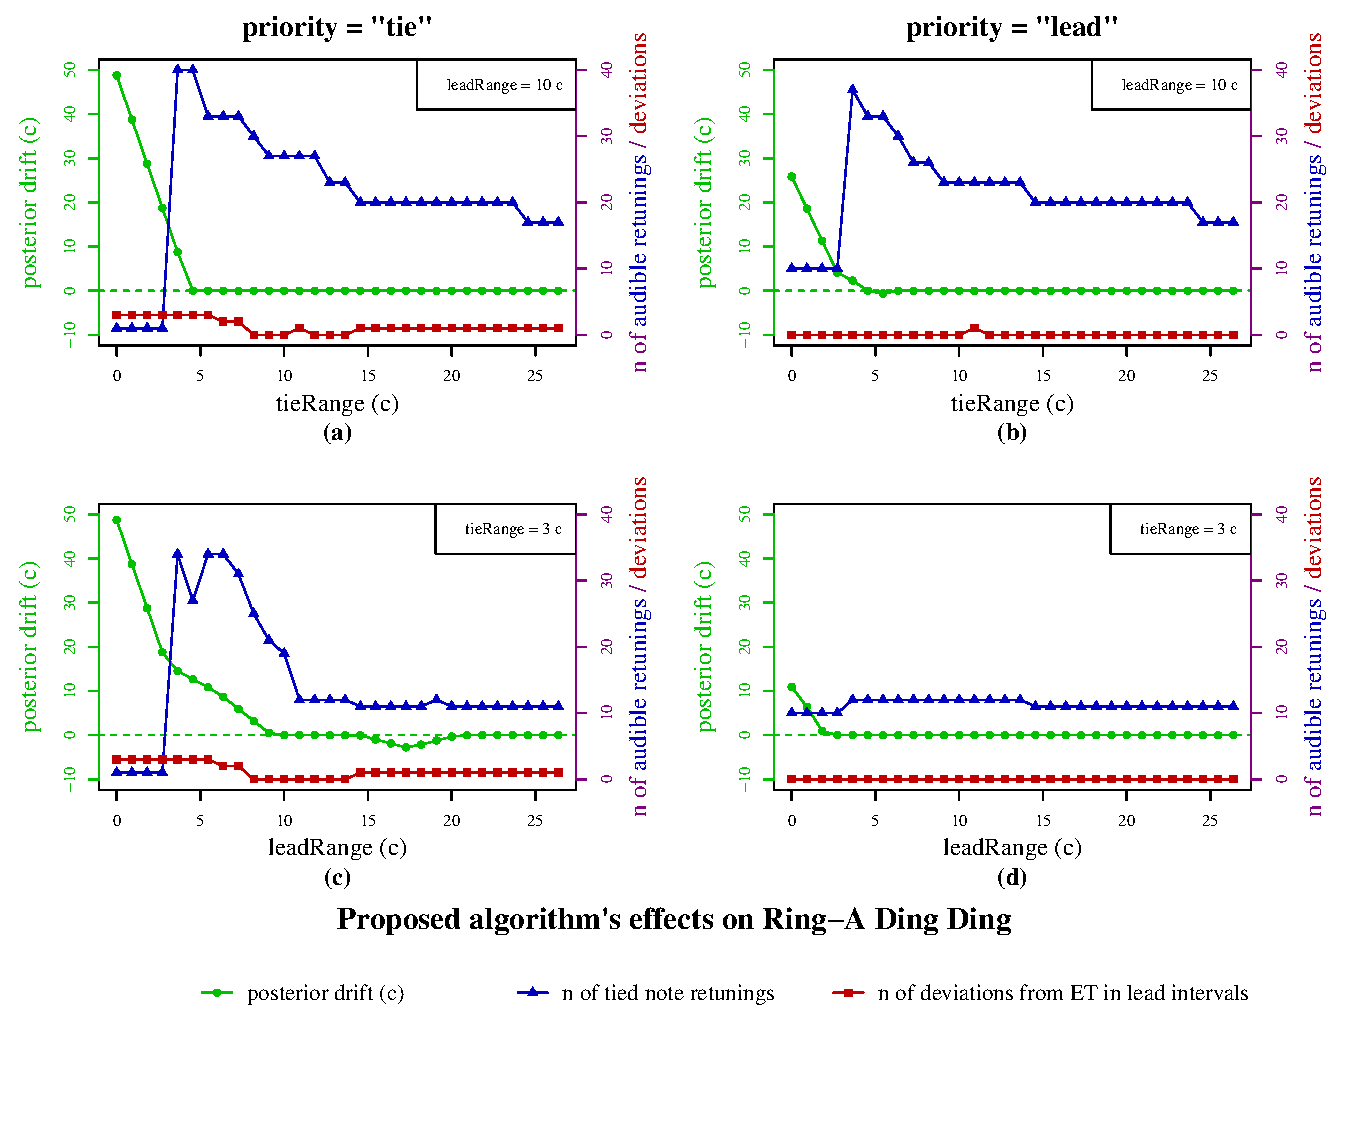
\includegraphics[width=\linewidth]{Results/effects_ring.pdf}
	\caption{Results from the proposed algorithm on the tag of Ring-a-Ding-Ding (sheet music in Figure \ref{fig:ding_sheets}). The graphs show the effects of parameter changes (x-axis) on three measures (y-axes): overall tonal centre drift in cents (green), number of tied note retunings over 3 cents (blue) and number of deviations from equal temperament in the lead voice larger than 10 cents (red). The tieRange and leadRange parameters determine how loosely the algorithm allows the most important held notes to retune (tie constraint) and how loosely it allows the lead voice's intervals to deviate from equal temperament. The left two graphs have the \textit{priority} set to "tie", whereas the right two graphs have it set to "lead". Both parameters appear to have a similar effect on how many notes need to retune, how many lead intervals are outside equal temperament and how much the song drifts overall.}
	\label{fig:results}
\end{figure}

\section{Discussion}
\label{discussion}
\subsection{Results evaluation}
% Was het goed?
% TODO Iets met dat dit best oké is, logisch dat er zo'n sprong in de blauwe lijnen zit want dat is waar het algoritme het oké gaat vinden dat tied notes volledig herstemmen. Iets van discussie over dat drift steeds lager wordt als je minder streng bent, maar dat betekent dus wel dat alle noten een beetje meh herstemd moeten worden. Oeps, dat laatste kun je eigenlijk nog niet zo goed zien in het grafiekje
% Interessant: dipje in groen bij leadRadius = 17

% Antwoord vraag A: is dit het ideale algoritme? niet per se, je kunt nadenken over tie retunings eens per maat ofzo. maar 
Research question A was: {\it what adaptive tuning algorithm would a mathematically ideal barbershop quartet follow, given a score?} In this thesis project, an algorithm was proposed as the ideal tuning system for barbershop quartets, immediately approaching an answer to this question. However, the results show that there is no definitive answer to question A; it is impossible to tune the \textit{Ring-a Ding Ding} tag in such a way that all four constraints from Section \ref{methodoloy} are completely satisfied.

% Antwoord vraag B: is het succesvol geïmplementeerd? Ja!
Research question B was: {\it can we implement the tuning system from question A so that it models the ideal barbershop quartet?} The algorithm was successfully implemented in C$\sharp$, making the answer to question B a definitive yes. Of course, whether this implemented algorithm sounds like the perfect barbershop quartet is a matter of opinion. Nonetheless, since every chord is in just intonation and overall pitch drift can be kept to a minimum, it can be said that this algorithm poses a \textit{mathematically ideal} solution to the tuning problem that is implicitly posed by the Barbershop Harmony Society's Handbook. \cite{barbershop_harmony_society_contest_2022}

The results from Figure \ref{fig:results} show that completely satisfying the four constraints posed in Section \ref{methodoloy} is, as predicted, not possible with the proposed algorithm. When $\mathit{tieRange}$ and $\mathit{leadRange}$ are close to 0, the tie constraint is satisfied, but we land on a different tonal centre than we started on, meaning the drift constraint is not satisfied. With looser ranges, the drift constraint can be satisfied, but there will always be some tied notes that need to be retuned, meaning the tie constraint has to be let go. Different barbershop songs may give different results. \textit{Ring-a-Ding Ding} is a relatively hard song to tune, meaning it might be possible to find a satisfactory tuning for some common barbershop songs. More examples of songs can be found on the algorithm's \href{https://github.com/teuncb/adaptivebarbershop}{GitHub page}.

% Interesting stuff in the results: dipje in LO rood, 
A few interesting remarks can be made about the results from Figure \ref{fig:results}. Firstly, a very low $\mathit{tieRange}$ actually causes a very high number of retuned tied notes over 3 cents. That is because the algorithm prioritises tied notes in the order lead-bass-baritone-tenor; if the bass and tenor are both holding a note, then the tenor note might be completely ignored to ensure the bass note does not need to be retuned. Therefore, if the algorithm is very strict about the bass retuning, the tenor will only need to be retuned even more. Secondly, a steady $\mathit{tieRange}$ and a $\mathit{priority}$ set to lead appears to be a simple way to get a relatively low number of tied note retunings, because the lead interval can always be satisfied. Lastly, when the $\mathit{priority}$ is set to "tie", there is a certain area of $\mathit{tieRange}$ and $\mathit{leadRange}$ values where not a single lead interval has to deviate from equal temperament, even though both lower and higher values for the Range parameters cause some deviations to occur. The exact reason for this dip is unclear, but it most likely also has to do with the effects of the algorithm's priorities.

\subsection{In musical contexts}
% Is zo'n algoritme wel realistisch? Iets met een cognitief model
% Hagerman citaties; Bye Bye Pythagoras: is JI wel beter?
% 12-toonsstemming is niet overal het best; andere approach is Sethares
The use of a model such as the one proposed is debatable. For human performers, this algorithm would be impossible to realise; the exact calculations required would be too complicated to carry out while singing and the tiniest intonation changes cannot be replicated using the human voice. Also, the algorithm's goal is not to "capture theories of cognitive functioning in mathematical or computational form", which means it is not exactly a cognitive model. \cite{van_maanen_interpretation_2021} However, the algorithm's results could serve as a reference for real singers to hear what a potentially ideal method of tuning could be. Additionally, high-level findings from the algorithm such as described in section \ref{results} could give singers a frame of reference as to how they should generally tune their notes in a barbershop context.

Even the concept of just intonation itself is a subject of debate: are the intervals from the harmonic series really the best way to tune? Hagerman \& Sundberg analysed recordings of barbershop quartets and found that the tenor, baritone and bass use the lead as a reference to adjust their pitches, but their intervals often deviate from just intonation. \cite{hagerman_fundamental_1980} Thanks to new technologies in music information retrieval, intonation and drift in choirs have been analysed in recent years. \cite{devaney_study_2012, mauch_intonation_2014, dai_intonation_2019} Results from these analyses have even led some researchers to conclude that just intonation as a whole is not the ideal tuning method. \cite{parncutt_psychocultural_2018} However, not enough research has been done to completely isolate these findings from twelve-tone bias.

At the same time, it is important to note that twelve-tone bias does play a role in this article's proposed tuning system. Barbershop music is composed with the standard twelve-tone tuning system in mind and this algorithm does tend to return to them as a result of the lead and drift constraints. A tuning method that does not adhere to the twelve-tone system and is, therefore, more culturally independent, was proposed by Sethares. Instead of using fractions from the harmonic series, he proposes to analyse a note's timbre using its \textit{dissonance curve}. \cite{sethares_adaptive_1994} However, since this article focuses specifically on barbershop, dissonance curves will always adhere to the natural harmonic series and using the twelve-tone system is commonplace. For these reasons, it was decided not to use Sethares' proposal in the current research.

\subsection{Philosophical Framework}
\textit{\color{red}Hier kan ik schrijven over ethische consequenties en het verschil tussen strong en weak AI. Dat ga ik alleen nog doen als ik tijd over heb.}

\subsection{Future Work}
% MIDI Input of op z'n minst abc-notatie
% Analyse van echte barbershopintonatie (AMPACT, devaney)
The input for this algorithm was a newly-defined language, described in Appendix \ref{input}. Translating a score into this language has turned out to be a painstaking process and could be optimised better. One more common way to describe music in plain text is abc notation, which also allows chord annotation. \cite{walshaw_abc2mtex_1997} However, since automatic chord recognition has improved in the past couple of decades \cite{burgoyne_cross-validated_2007}, an implementation of this algorithm could easily be built that simply takes MIDI as input. Essentially, the only thing that the tuning system has to add is pitch bend messages.

The scope of this paper did not allow for a comparison to real-world barbershop quartets. In recent years, systems such as AMPACT can be used to evaluate the tuning tendencies of real choirs. \cite{devaney_study_2012} Analysing the difference between mathematically ideal algorithms such as the one proposed and the tendencies of professional barbershop quartets could lead to an even better tuning system. Eventually, a tuning system might be developed that all barbershop musicians can refer to when singing their genre.

\subsection{Code Availability}
All code for the C$\sharp$ implementation of the algorithm, along with example songs, source files for the images and \TeX-files for this paper can be found on \texttt{\url{https://GitHub.com/teuncb/AdaptiveBarbershop}}.

% TODO referenties naar webpagina's fixen
\bibliography{AdaptiveBarbershop.bib}

\begin{appendices}

\section{Input language}
\label{input}

\textit{\color{red}Ook dit ga ik nog schrijven en ook dit is niet zo interessant. Je kunt de informele specificatie voor nu alvast \href{https://flashy-suit-0e2.notion.site/C-parser-bouwen-e9ba52712772466d846865649184b58f}{op Notion (klik!)} vinden.}
\subsection{Songs}
\label{input_songs}
% Notes: n, b and #; octaves; tied notes
% Chords: with 4 notes, sometimes not playing; chord symbols
% duration in MIDI, timecode at 480 (find unit)
\subsection{Fractions}
\label{input_fractions}
% slashes

\end{appendices}

\end{document}